% Links
% Mathematics of infectious diseases https://epubs.siam.org/doi/10.1137/S0036144500371907

\chapter{Modelling infectious diseases}
\label{chapter:modelling_of_infectious_diseases}
The purpose of this chapter is to get a grasp of how infectious diseases can be modelled to obtain relevant information through simulations. Therefore, a good understanding of infectious diseases and how they can spread is needed, and thus explained first. Then, the architectural design behind such models is described with regard to how Stride is designed. It must be stated that this chapter's intent is solely to present information collected from academic publications and literature that is considered relevant for this thesis. It does therefore not contain any sort of new personal research, neither is it an examination of the given content. The content of this chapter is based on \cite{book:principles_infectious_diseases, book:transmission_principles, contact_tracing_and_disease_control, innate_immunity, acquired_immunity, types_of_immunity, acute_infections, sir_model_origin, book:modelling, usefulness_models, stochastic_modelling, compartmental_model, lander_lessons_decade, lander_phd, introduction_agent-based_models, abm_surging_tool, abm_methods_and_techniques, parameter_importance_bilcke, lander_estimating}.

\begin{figure}[ht]
    \centering
    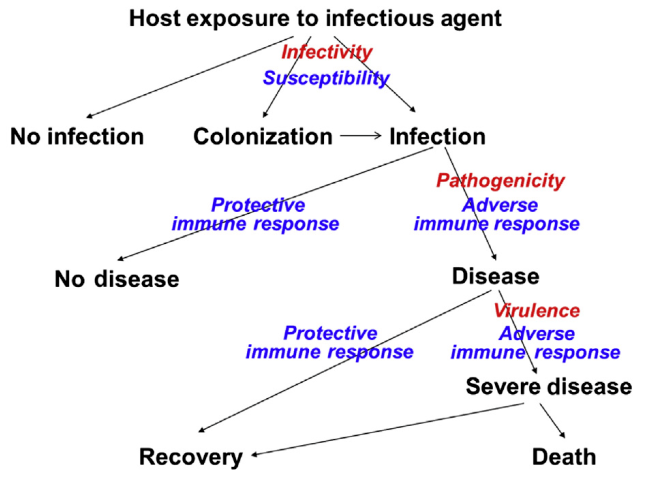
\includegraphics[width=.5\textwidth]{2 - Modelling of infectious diseases/fig/infectious_disease_outcomes.png}
    \caption{Potential outcomes of a host exposed to a pathogen (infectious agent) with depending factors of progression between stages. Figure copied from \cite{book:principles_infectious_diseases}.}
    \label{fig:infectious_disease_outcomes}
\end{figure}

\section{Concepts of infectious diseases}
\label{sec:concepts_of_infectious_diseases}
An infectious disease is an illness caused by any sort of pathogen, including bacteria and viruses, which is transferred from one host to another. Transmission of pathogens can occur in various ways, which is explained in Section \ref{subsec:transmission}, but does not necessarily mean that the new host will become ill. Figure \ref{fig:infectious_disease_outcomes} illustrates that exposure of a host to a pathogen can result in different outcomes. These outcomes are dependent on numerous factors such as the host's susceptibility to infection and disease, environmental factors, and physical and social behaviour of the host. If a new pathogen reaches a new host, it starts to colonize: multiplication of the pathogen at an entry point such as the skin or the mucous membranes of the respiratory, digestive, or urogenital tract. Then the pathogen starts to invade and establish within the host's tissue and causes disruption within a host, but does not necessarily result in disease. Clinical disease only occurs when a certain level of disruption has been reached which translates into symptoms and signs of illness. The final outcome of the disease varies in every situation, in which the immune system of the host plays a major role in. Depending on the host's immune system and the disease, the host may maintain immunity to the disease \cite{book:principles_infectious_diseases}.

\subsection{Transmission}
\label{subsec:transmission}
An important trait of many infectious diseases is that an infected host can act as a source of exposure to others. As will be explained in Chapter \ref{chapter:stride}, Stride focuses primarily on air-borne diseases such as measles, influenza, and COVID-19 which are mainly transmitted through means of direct contact. This thesis will thus concentrate on transmission through contact. For the sake of completeness however, we mention that there are five distinct means of transmission \cite{book:transmission_principles}:

\begin{enumerate}
    \item Through contact, direct (skin or sexual contact) or indirect (infected fomite, blood or body fluid). Inhaling contaminated air also falls into this category
    \item Ingesting contaminated food.
    \item Through vectors (mosquito, tick, etc.).
    \item Through pregnancy.
\end{enumerate}

\subsection{Stages}
\label{subsec:stages}
When a transmission of a pathogen has occurred, the exposed individual can become ill as discussed earlier. This does not mean that the recently infected person immediately becomes infectious to others or starts showing symptoms. Infectious diseases have different stages and the duration of those stages is different depending on the person and the type of infection, among other things. The time from exposure until the time of the first signs of symptoms of disease is called the \textit{incubation period}. After the incubation period, the \textit{period of clinical illness} starts which describes the duration between the first and last signs or symptoms. These periods are used to describe how the disease manifests itself to the infected person, but they do not say anything about the infectiousness of the infected person. The term to describe the time from exposure until the onset of infectiousness is the \textit{latent period}. The latent period is followed by the \textit{infectious period} which is the duration when the infected person can transmit pathogen. Figure \ref{fig:stages_infectious_diseases} visualises these periods for different types of diseases. It should be noted that these periods are an indication and that they can vary from person to person.  \cite{book:principles_infectious_diseases}
\\\\
The most obvious pattern of these stages is when the incubating and latent period are the same, as well as the clinical ill and infectious period. An example of such a disease is Ebola, and is shown in Figure \ref{subfig:stages_ebola}. Diseases where these patterns nicely follow up on each other are relative easy to treat and predict individually. Unfortunately there are also diseases where this is not the case.

\begin{figure}[!ht]
\centering
\begin{subfigure}[!ht]{\textwidth}
    \centering
    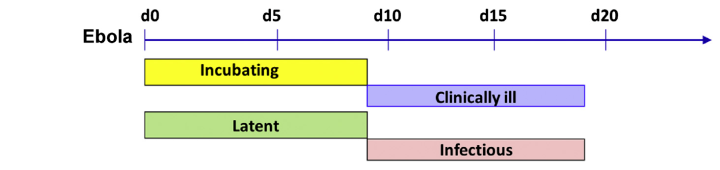
\includegraphics[width=.7\linewidth]{2 - Modelling of infectious diseases/fig/stages_ebola.png}
    \caption{}
    \label{subfig:stages_ebola} 
\end{subfigure}

\begin{subfigure}[!ht]{\textwidth}
    \centering
    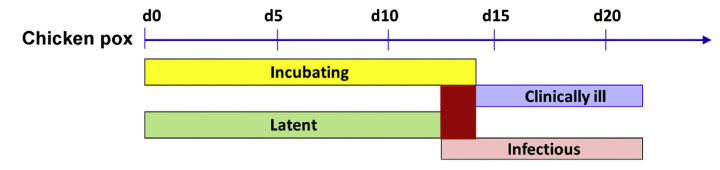
\includegraphics[width=.7\linewidth]{2 - Modelling of infectious diseases/fig/stages_chicken_pox.png}
    \caption{}
    \label{subfig:stages_chicken_pox}
\end{subfigure}

\begin{subfigure}[!ht]{\textwidth}
    \centering
    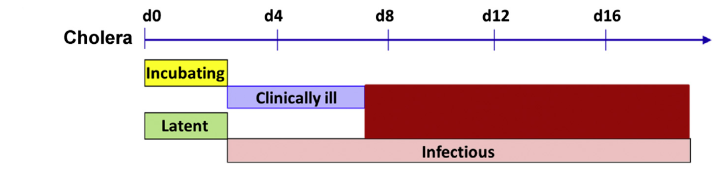
\includegraphics[width=.7\linewidth]{2 - Modelling of infectious diseases/fig/stages_cholera.png}
    \caption{}
    \label{subfig:stages_cholera}
\end{subfigure}

\begin{subfigure}[!ht]{\textwidth}
    \centering
    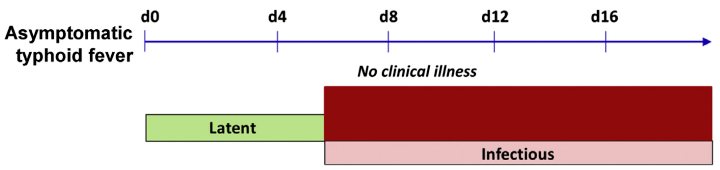
\includegraphics[width=.7\linewidth]{2 - Modelling of infectious diseases/fig/stages_asymptomatic_typhoid_fever.png}
    \caption{}
    \label{subfig:stages_asymptomatic_typhoid_fever}
\end{subfigure}

\caption[Stages of infectious diseases]{Stages of infectious diseases for different types of disease in function of the time since exposure (in days). The red bar displays when an infectious person is asymptomatic infectious. Figure copied from \cite{book:principles_infectious_diseases}.}
\label{fig:stages_infectious_diseases}
\end{figure}

\subsection{Asymptomatic carrier}
\label{subsec:asymptomatic_carrier}
It is possible that a person is infectious to others, but yet shows no signs or symptoms of disease. Someone who satisfies these conditions is called an \textit{asymptomatic carrier}, which can be divided in three different types of carrier \cite{book:principles_infectious_diseases}:
\begin{enumerate}
    \item \textbf{Incubatory:} This occurs when the incubation period overlaps with the infectious period and is for example the case with chicken pox, shown in Figure \ref{subfig:stages_chicken_pox}.
    \item \textbf{Convalescent:} In this case the clinically ill period ends before the infectious period. Cholera is such a disease and is visualised in Figure \ref{subfig:stages_cholera}.
    \item \textbf{Healthy:} This is the case when someone has no signs or symptoms, but still can infect others like with asymptomatic typhoid fever shown in Figure \ref{subfig:stages_asymptomatic_typhoid_fever}.
\end{enumerate}
It is clear that asymptomatic carriers make it harder to contain a disease. When treating infectious diseases it is therefore important to know when the different stages appear in order to take the appropriate actions such as contact tracing and isolation \cite{contact_tracing_and_disease_control}.

\subsection{Immunity}
\label{subsec:immunity}
Prevention of a disease can be more important than a cure, especially when trying to control an outbreak. Being immune to a disease therefore offers the best solution in prevention from getting ill. The actual workings of immunity will not be explained as they do not add value to this thesis. The different ways to become immune, however, deserve some elaboration to give insight in how this can effect the modelling of infectious diseases.
\\\\
The first case is called \textit{innate} immunity, which describes the immunity someone is born with \cite{innate_immunity}. The second case is \textit{adaptive} or \textit{acquired} immunity, and is used to denote the cases of immunity that are gained after being born. Once born, immunity can be acquired in four different ways as shown in Figure \ref{fig:immunity}. A distinction can be made between \textit{active} and \textit{passive}, and between \textit{natural} and \textit{artificial} immunity. Active immunity is gained when exposure to a pathogen triggers the immune system to produce antibodies for that pathogen, while passive immunity is gained when someone receives antibodies without being exposed to a pathogen. Active immunity can occur in a natural way when infected by a pathogen, or in an artificial manner when vaccinated. Likewise, passive immunity can happen in a natural way by receiving antibodies through breastfeeding or the placenta, or in an artificial way through globulin \cite{types_of_immunity}.

\begin{figure}[ht]
    \centering
    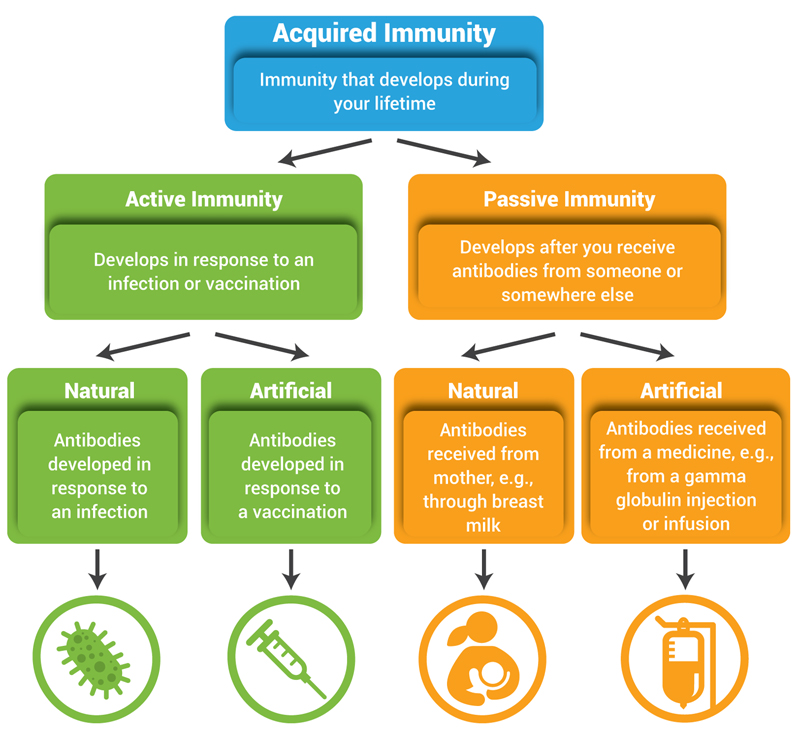
\includegraphics[width=.6\textwidth]{2 - Modelling of infectious diseases/fig/immunity.jpg}
    \caption{A visualization of the different types of acquired immunity. Figure copied from \cite{acquired_immunity}.}
    \label{fig:immunity}
\end{figure}

\subsection{Acute versus chronic}
\label{subsec:acute_vs_chronic}
The last thing that has to be discussed about infectious diseases is the different types of infection. The two most used terms to describe infections are \textit{acute} and \textit{chronic infections} and their key distinction is the duration of the infection. An acute infection lasts no more than six months, whilst a chronic infection lasts longer than six months. Also, the symptoms of acute infections develop rapidly over the course of days, in contrast to chronic infections where symptoms develop over weeks or months. Measles and influenza, the diseases Stride focuses on, are caused by acute infections. Therefore, whenever infectious diseases are mentioned in this thesis, they refer to those that are cause by acute infections \cite{acute_infections}.

\section{Mathematical models of infectious diseases}
A model is used as a representation of something and can be used by anyone in any field, with for example an architect who can build a scale model to represent their idea of a building. The architect's scale model can be just four walls and a roof, or the architect may have put incredible attention to detail in his work with by decorating every room. The difference in both models lies in the amount of work done by the architect. Likewise, a model to simulate infectious diseases can be a fast high-level program that produces little information, or a very complex program that needs a substantial amount of time to calculate detailed information of every individual. The next step in building such a model, is thus to understand how the recently gathered knowledge about infectious diseases can be applied and what trade-offs have to be made to get the desired results.

%\subsection{Basic reproduction number}
%Before moving on to the models, the basic reproduction number (denoted by $R_0$) needs a brief explanation. The number is a metric used to describe the contagiousness of a disease. Concretely, it represents the number of people that one infectious person will directly infect over the course of their infection, when placed in a fully susceptible population. \cite{r0}

\subsection{SIR model}
\label{subsec:sir_model}
Section \ref{subsec:acute_vs_chronic} explained that the focus lies on infectious diseases caused by acute infections, and thus the different stages of infectious diseases from Section \ref{subsec:stages} are short periods of time. Section \ref{subsec:transmission} also explained that the only type of transmission that will be considered is through contact. With this information, the most basic transmission model for a transmitted infectious disease can be used, called the SIR model which refers to its three compartments: susceptible, infected, and recovered. It is a system that consists of three coupled non-linear ordinary differential equations. The model makes use of very strict assumptions and is therefore not an abstract representation of the real world. There are numerous variations on the SIR model with different assumptions, but the basic assumptions are the following:
\begin{itemize}
    \item A large, fixed population represented as one large group, so without subgroups, where no demographic events occur.
    \item The infection has no latent period, thus an individual becomes infectious as soon as they become infected.
    \item Once someone is recovered, they are forever immune.
    \item Every person can encounter every other person with the same probability each day (which has nothing to do with probabilities, but rather with an intuitive model).
    \item The outbreak is normally short lived, but this can also be changed depending on the specified parameters.
\end{itemize}

\noindent Although the model makes strong assumptions, it still provides a lot of value. With simple calculus, a great deal of information can be extracted such as the reproductive number of the disease, the rate of recovery, and the rate of infection \cite{sir_model_origin}.

\subsection{SEIR model}
\label{subsec:seir_model}
An aspect of the SIR model is that there is no latent period. However, Sections \ref{subsec:stages} and \ref{subsec:asymptomatic_carrier} showed that the latent period is an important part of infectious diseases. In order for a model to give a more accurate representation of infectious diseases, it thus needs to take this period into account. The SEIR model is a refinement of the SIR model that fulfills this need by adding the \textit{exposed} state between the susceptible and infectious states. The exposed state represents the latent period when someone has been exposed to pathogen, but in which the amount of pathogen is too low in order for the host to infect others. Figure \ref{fig:seir-model} illustrates how the exposed state gives the SEIR model a more accurate representation of infectious diseases \cite{book:modelling}.

\begin{figure}[ht]
    \centering
    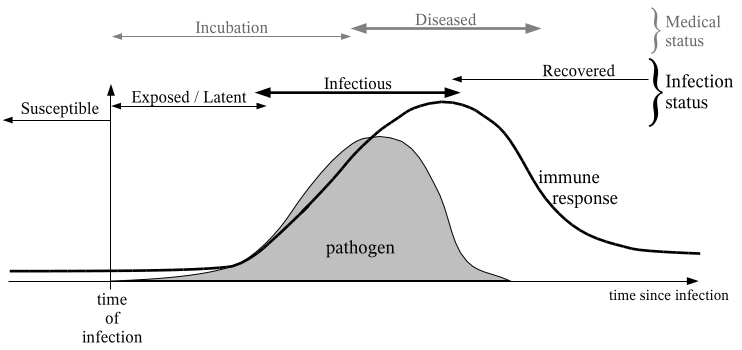
\includegraphics[width=\textwidth]{2 - Modelling of infectious diseases/fig/infection_timeline.png}
    \caption{A generalized representation of an infection over time, showing the different stages related to the dynamics of the pathogen and the host's immune response. Figure copied from \cite{book:modelling}.}
    \label{fig:seir-model}
\end{figure}

\subsection{Additional refinements}
The SEIR model is more advanced than the SIR model, but it is far from perfect. Section \ref{subsec:immunity} explained how immunity can be achieved in different ways. Further refinement of these models would thus be to incorporate the possibility of people being born with immunity. Since people do not necessarily become immune to a disease once they have recovered from it, another refinement would be to add the possibility of people becoming susceptible instead of immune after recovery. A third refinement could satisfy the lack of asymptomatic carriers, which is explained in Section \ref{subsec:asymptomatic_carrier}, by adding the possibility of people being an asymptomatic carrier \cite{book:modelling}.

\subsection{Deterministic and homogeneous}
\label{subsec:deterministic_and_homogeneous}
The models that have been explained could be seen as deterministic models. Given the same starting conditions, they would produce the same results every time. These models are limited to uniform and homogeneous populations, but still provide useful insights in infectious diseases \cite{usefulness_models}. However, their resemblance of the real world lacks the structure and stochasticity of every day life. In real life, people are divided in sub-populations such as their household, workplace, and school, where they meet different people every day. Every decision someone makes can have an impact on what their next decision will be or even what someone else their decisions will be. In order to simulate real life, different decision outcomes need to be taken into account. The simulation of such a decision can be seen as the collection of every possible outcome, for which every outcome has a probability that it will happen. This role of chance has a big impact when the number of infected people is relatively small or when considering a small (sub-)population \cite{stochastic_modelling}.

\section{Computational model simulations}
\label{sec:computational_model_simulations}
Every simulation serves a certain purpose, and so computational models can be designed in different ways to serve different purposes. This last section of the introductory chapter explains, based on Stride, how a computational model can be build to simulate infectious diseases. 

\subsection{Individual-based models}
\label{subsec:individual-based_models}
Section \ref{subsec:deterministic_and_homogeneous} explained how the mathematical models give a more high-level representation of infectious diseases in a population. One of their concepts is that they make use of homogeneous populations, which states that everyone in the population is and acts completely the same. Their results show the transmission dynamics based on the amount of people in every compartment (susceptible, infected and recovered), which only tells something on a population-level \cite{compartmental_model}. These results thus do not tell anything about the individuals that get infected or who someone has contacts with. If such more detailed results are required, a different model design is needed.
\\\\
These details cannot be gathered from a homogeneous population model, because everyone is then the same and no distinctions can be made. A heterogeneous population is needed which is when there are distinct individuals each with their own `life'. These distinctions can be made based on age, places they visit, people they meet, and so on. Every individual has thus their own identity and information that needs to be captured as well as the interactions with everyone else. A model that fulfills these needs is an individual-based model of which the definition is given by Willem et al. \cite{lander_lessons_decade, lander_phd}:
\begin{quoting}
"A computer simulation for the creation, disappearance and movement of a finite collection of interacting individuals or agents with unique attributes regarding spatial location, physiological traits and/or social behaviour."
\end{quoting}

In an individual-based model the population is designed in a bottom-up fashion. The population-level information is now the result of all the interactions between the individuals and their `behaviour' \cite{lander_lessons_decade}. Behaviour of individuals can also change based on for example different days of the week (weekday and weekend), or when feeling ill. It also allows for different environments to be created where every environment has its own type of behaviour \cite{introduction_agent-based_models}.

\begin{example}
\label{example:different_behaviour}
When at work, people interact very different than when they are at home. When at home, the contacts between people are closer than those at work. As such, individuals in different environments will `act' in different ways.
\end{example}

\noindent These environments also give the possibility to incorporate different stochastic interactions for each environment, which is very valuable when looking smaller populations as was stated in Section \ref{subsec:deterministic_and_homogeneous}.

\begin{example}
\label{example:different_stochasticity}
An infectious person has a much higher probability of infecting members of their household than colleagues at work.
\end{example}

Additionally, these models can give the option to track every individual in as much detail as desired. This gives the possibility to create a `history' for every individual as well as their network of contacts, thus providing new information in understanding different phenomena \cite{lander_lessons_decade}.
\\\\
Overall, as stated by Murphy et al. \cite{introduction_agent-based_models}, these models can be of use in countless situations to provide insights into the adaptation and function of systems. Another important asset of them is that they grant these insights when access to field data is dangerous, unavailable, or impossible to collect, with for example the COVID-19 pandemic that made collecting field data extremely difficult. Furthermore, research with individual-based models is a growing community, where open-source information and software play an important role. This, together with the increasing computational power, ensures future improvements in this field \cite{introduction_agent-based_models, abm_surging_tool}.

\subsection{Parameterization}
\label{subsec:parameterization}

Next to creating a model, parameters that are passed to the simulation need to be established. It is obvious that parameters can greatly impact the results of a simulation and thus definitely need to be chosen carefully:

\begin{example}
Looking back at Examples \ref{example:different_behaviour} and \ref{example:different_stochasticity}, the different probabilities in every environment need to be defined with actual values. If the probability that someone acquires an infection is slightly higher or lower, it can result in respectively more or less infected people in a simulation.
\end{example}

There are numerous ways to gather the required data with open-source data proving a valuable asset in these situations. In some cases it might be challenging, because certain interactions may not exist or still need some research \cite{abm_methods_and_techniques}. When parameters need to be estimated, there is a level of uncertainty that needs to be accounted for. Various techniques have been presented to give more accurate estimations on parameters \cite{lander_understand_models, parameter_importance_bilcke}, with a more relevant study about transmission model parameters for seasonal influenza by Willem et al. \cite{lander_estimating}. What parameters and data are being used in Stride, will be seen in the next chapter.
